% Retrieval as ranking — TikZ source. Compiles to a tight standalone PDF
% (pdflatex figures/retrieval-rank.tex), which `book-scaffold build-figures`
% converts to public/figures/retrieval-rank.svg.
%
% Candidates sorted by similarity to the query; the true match (highlighted)
% lands in the top-k band. recall@1 = true match is first; MRR rewards low rank.
\documentclass[tikz,border=3pt]{standalone}
\usepackage{amsmath}
\usepackage{amssymb}
\usepackage{tikz}
\usetikzlibrary{positioning,arrows.meta,calc}
\begin{document}
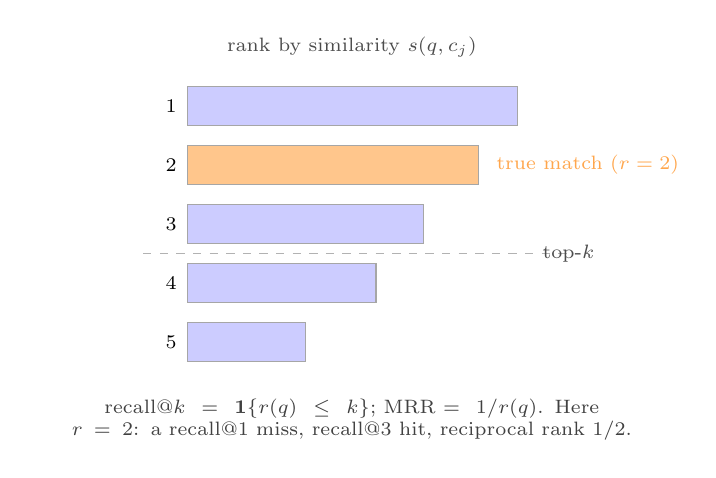
\begin{tikzpicture}[
    font=\small,
    bar/.style={draw, gray!70, fill=blue!20, minimum height=5mm, inner sep=1pt,
                anchor=west},
    hit/.style={draw, gray!70, fill=orange!45, minimum height=5mm, inner sep=1pt,
                anchor=west},
  ]
  % sorted similarity bars (decreasing); the true match is rank 2 here
  \node[bar, minimum width=42mm] (c1) at (0,0) {};
  \node[hit, minimum width=37mm] (c2) at (0,-0.75) {};
  \node[bar, minimum width=30mm] (c3) at (0,-1.5) {};
  \node[bar, minimum width=24mm] (c4) at (0,-2.25) {};
  \node[bar, minimum width=15mm] (c5) at (0,-3.0) {};

  \node[left, font=\scriptsize] at (0,0) {1};
  \node[left, font=\scriptsize] at (0,-0.75) {2};
  \node[left, font=\scriptsize] at (0,-1.5) {3};
  \node[left, font=\scriptsize] at (0,-2.25) {4};
  \node[left, font=\scriptsize] at (0,-3.0) {5};
  \node[right=1mm of c2, font=\scriptsize, text=orange!70] {true match ($r=2$)};

  % top-k band (k=3)
  \draw[gray!60, dashed] (-0.55,-1.875) -- (5.0,-1.875);
  \node[right, font=\scriptsize, text=black!70] at (4.4,-1.875) {top-$k$};

  \node[above, font=\scriptsize, text=black!70] at (2.1,0.5) {rank by similarity $s(q,c_j)$};
  \node[below, align=center, text width=8cm, font=\scriptsize, text=black!75]
    at (2.1,-3.6)
    {recall@$k=\mathbf 1\{r(q)\le k\}$; MRR $=1/r(q)$. Here $r=2$: a recall@1 miss,
     recall@3 hit, reciprocal rank $1/2$.};
\end{tikzpicture}
\end{document}
